\documentclass[a4paper]{llncs}
\usepackage[T1]{fontenc}
\usepackage[utf8]{inputenc}
\usepackage[portuguese]{babel}
\usepackage{lmodern}
\usepackage{booktabs}
\usepackage{tabularx}
\usepackage{graphicx}
\usepackage{xcolor}
\usepackage{fancyvrb}
\usepackage{tikz}
\usetikzlibrary{arrows.meta,fit,positioning}

\renewcommand{\keywordname}{{\bf Palavras-chave:}}
\renewcommand{\andname}{e}
\renewcommand{\lastandname}{\unskip\ e}
% Sem cabeçalhos corridos; apenas o número de página no rodapé.
\pagestyle{plain}
\raggedbottom
\setlength{\tabcolsep}{4pt}
\newcolumntype{L}[1]{>{\raggedright\arraybackslash}p{#1}}
\newcolumntype{Y}{>{\raggedright\arraybackslash}X}
\setlength{\textfloatsep}{8pt plus 2pt minus 2pt}
\setlength{\floatsep}{6pt plus 2pt minus 2pt}
\setlength{\intextsep}{7pt plus 2pt minus 2pt}
% Excertos de código e de consola.
\DefineVerbatimEnvironment{code}{Verbatim}{fontsize=\scriptsize, frame=single,
  framesep=3pt, samepage=true,
  listparameters={\setlength{\topsep}{4pt}\setlength{\partopsep}{0pt}},
  rulecolor=\color{black!40}, xleftmargin=1pt, xrightmargin=1pt}
\graphicspath{{../../results/full/figures/}{../progresso/figuras/}}

\begin{document}

\title{Implementação de mecanismos de QoS\\ usando VNFs\\{\large Relatório final --- TP3}}

\author{André Miguel Rego Trindade Pinto \and Diogo Fernandes Pinto \and\\ Francisco José Fidalgo Lage}

\institute{Grupo PL11 --- Qualidade de Serviço na Internet,\\ Universidade do Minho, Braga, Portugal\\
\email{\{pg65400, pg65405, pg65407\}@alunos.uminho.pt}}

\maketitle

\begin{abstract}
Este trabalho implementa e avalia um sistema de QoS do tipo DiffServ em que cada função
de rede é uma VNF: um contentor Docker que usa mecanismos do \emph{kernel} Linux.
Quatro VNFs em cadeia cobrem os cinco aspetos de QoS do enunciado: classificação,
controlo de acesso, policiamento, agendamento e monitorização. O sistema corre sobre
uma topologia emulada com um gargalo de 10~Mbit/s e é avaliado com tráfego VoIP, de
vídeo e de dados em massa, numa campanha automática de 420~corridas. Com a cadeia
ativa, o atraso do VoIP desce de 109~ms para 5~ms e deixam de existir perdas em VoIP e
vídeo, com um custo de 4\% no débito TCP. O relatório quantifica ainda o contributo de
cada VNF, os compromissos da otimização e a sobrecarga da virtualização.
\keywords{QoS \and NFV \and VNF \and DiffServ \and Cadeia de serviço \and Token bucket \and HTB}
\end{abstract}

\section{Introdução}

A qualidade de serviço (QoS) na Internet foi durante muito tempo garantida por
equipamento dedicado: encaminhadores com listas de acesso, policiadores e filas
implementados em \emph{hardware}. A virtualização de funções de rede (NFV) separa
essas funções do equipamento e passa a executá-las como \emph{software}, as VNFs, em
servidores comuns~\cite{etsi-nfv}. Ganha-se flexibilidade, porque uma função pode ser
criada, reconfigurada ou substituída em segundos, e paga-se um custo de desempenho,
porque cada pacote atravessa mais \emph{software}.

O objetivo deste trabalho é conceber, implementar e otimizar um sistema de QoS baseado
em VNFs e medir o que ele vale. As perguntas a que o relatório responde são três:
(i)~quanto melhora cada VNF as métricas de QoS do tráfego multimédia, e à custa de
quê; (ii)~como devem ser escolhidos os parâmetros dos mecanismos; (iii)~quanto custa
fazer isto com funções virtualizadas.

O sistema segue a arquitetura DiffServ~\cite{rfc2475}: o tráfego é classificado e
marcado à entrada, policiado segundo um perfil contratado e servido por classes no
ponto de congestionamento. Para ser simples de explicar e de reproduzir, cada VNF usa
apenas mecanismos nativos do Linux (\texttt{nftables} e \texttt{tc}), e todo o
ambiente, as experiências e os gráficos são criados por \emph{scripts}. O código, a
configuração e os dados estão em \texttt{https://github.com/Daydream127/Qosi}.

\section{Arquitetura e implementação}
\label{sec:arq}

\subsection{Topologia e ambiente}

A topologia (Fig.~\ref{fig:topo}) é semelhante à de um ISP pequeno e é emulada com o
Containernet~\cite{containernet}, uma extensão do Mininet~\cite{mininet} que usa
contentores Docker como nós. Quatro clientes ligam-se a um comutador Open~vSwitch
(s1). Todo o tráfego atravessa a cadeia de quatro VNFs antes de chegar ao encaminhador
do núcleo (r1) e, através de um segundo comutador (s2), aos três servidores. A saída
da VNF3 é o \emph{gargalo}, limitado a 10~Mbit/s: é o único ponto onde há contenção.
Na ligação ao núcleo, o \texttt{tc netem} acrescenta 5~ms de atraso em cada sentido e
permite emular mais atraso, perdas e falhas.

\begin{figure}[!tb]
\centering
\resizebox{\textwidth}{!}{%
\begin{tikzpicture}[font=\scriptsize, >=Latex,
  host/.style={draw, rounded corners=1pt, minimum width=1.3cm, minimum height=0.42cm, inner sep=1pt},
  sw/.style={draw, circle, inner sep=1.5pt, fill=gray!15},
  vnf/.style={draw, thick, fill=blue!8, minimum width=1.35cm, minimum height=1.0cm, align=center, inner sep=1pt},
  mgmt/.style={draw, fill=green!10, minimum height=0.5cm, inner sep=3pt, align=center}]
  \node[host] (hv) at (0,1.2) {h\_voip};
  \node[host] (hd) at (0,0.4) {h\_video};
  \node[host] (hb) at (0,-0.4) {h\_bulk};
  \node[host, densely dashed] (hx) at (0,-1.2) {h\_x};
  \node[above=1pt of hv, font=\scriptsize\itshape] {Clientes};
  \node[sw] (s1) at (1.4,0) {s1};
  \node[vnf] (c) at (2.9,0) {VNF1\\Classificador};
  \node[vnf] (f) at (4.6,0) {VNF2\\Firewall};
  \node[vnf] (p) at (6.3,0) {VNF3\\Policer/\\Scheduler};
  \node[vnf] (m) at (9.3,0) {VNF4\\Monitor};
  \node[draw, dashed, inner sep=5pt, fit=(c)(f)(p)(m),
        label={[font=\scriptsize\itshape]above:Cadeia de serviço (contentores Docker)}] (chain) {};
  \node[sw] (r1) at (11.6,0) {r1};
  \node[sw] (s2) at (12.5,0) {s2};
  \node[host] (sv) at (13.85,0.8) {srv\_voip};
  \node[host] (sd) at (13.85,0) {srv\_video};
  \node[host] (sb) at (13.85,-0.8) {srv\_bulk};
  \node[above=1pt of sv, font=\scriptsize\itshape] {Servidores};
  \foreach \h in {hv,hd,hb,hx} \draw (\h.east) -- (s1);
  \draw[->] (s1) -- (c);
  \draw[->] (c) -- (f);
  \draw[->] (f) -- (p);
  \draw[->, very thick] (p) -- node[above] {10 Mbit/s} node[below] {gargalo} (m);
  \draw[->] (m) -- node[above, pos=0.66] {netem} (r1);
  \draw (r1) -- (s2);
  \foreach \s in {sv,sd,sb} \draw (s2) -- (\s.west);
  \node[mgmt, minimum width=8.3cm] (prom) at (6.1,-1.75) {Prometheus + Grafana (rede de gestão)};
  \foreach \v in {c,f,p,m} \draw[dashed, ->, gray] (\v.south) -- (\v.south |- prom.north);
\end{tikzpicture}}
\caption{Topologia emulada e cadeia de serviço (h\_x é uma origem não autorizada).}
\label{fig:topo}
\end{figure}

O ambiente é um Ubuntu~22.04 com Containernet, Docker e Open~vSwitch, instalado por
um único \emph{script}. Em relação à proposta, a máquina virtual VirtualBox foi
trocada por uma distribuição dedicada no WSL2: com o Hyper-V ativo, a primeira era
demasiado lenta para medir atrasos com rigor.

\subsection{Cadeia de serviço e orquestração}

Em termos da arquitetura ETSI~NFV~\cite{etsi-nfv}, a infraestrutura (NFVI) é formada
pelo Docker, pelo Open~vSwitch e pelo Containernet, e as VNFs são os quatro
contentores da Tabela~\ref{tab:vnfs}. O papel de orquestrador é desempenhado, de
forma simplificada, por um \emph{script} (\texttt{topology/qosnet.py}), que lê a
configuração em \texttt{config/chain.yaml}, cria os contentores e as ligações, atribui
endereços e rotas e corre em cada VNF o \emph{script} \texttt{/vnf/start}, com os
parâmetros passados em variáveis de ambiente.

\begin{table}[!tb]
\caption{VNFs da cadeia, aspetos de QoS cobertos e ferramentas.}
\label{tab:vnfs}
\centering
\footnotesize
\begin{tabularx}{\textwidth}{@{}L{4.1cm} L{2.5cm} Y@{}}
\toprule
VNF e \emph{aspeto de QoS} & Ferramenta & Função \\
\midrule
1 Classificador\newline \emph{Classificação} & \texttt{nftables} &
  Identifica os fluxos por destino, protocolo e porta; marca o DSCP. \\
\addlinespace[2pt]
2 Firewall\newline \emph{Controlo de acesso} & \texttt{nftables} &
  Política \emph{default-deny}: só admite origens e serviços autorizados. \\
\addlinespace[2pt]
3 Policer/Scheduler\newline \emph{Policiamento, agendamento} & \texttt{tc} (police, HTB) &
  \emph{Token bucket} por classe à entrada; três classes HTB à saída. \\
\addlinespace[2pt]
4 Monitor\newline \emph{Monitorização} & \texttt{nftables}, Python, Prometheus, Grafana &
  Contadores por classe; métricas exportadas e visualizadas em tempo real. \\
\bottomrule
\end{tabularx}
\end{table}

O encadeamento é feito por encaminhamento, como numa cadeia de funções de
serviço~\cite{rfc7665} em linha: cada VNF tem duas interfaces de dados, é um salto IP
e encaminha para a seguinte. A ordem da cadeia é a da lista no ficheiro de
configuração, e os endereços e as rotas são gerados a partir dela; trocar a ordem ou
retirar uma VNF é editar esse ficheiro.

Um \emph{perfil} é um conjunto de alterações às variáveis das VNFs, também definido
no ficheiro de configuração (por exemplo, \texttt{SCHEDULING: 0} na VNF3). Aplicar um perfil
volta a correr os \emph{scripts} \texttt{start}; uma VNF desativada fica em modo de
passagem e limita-se a encaminhar. Assim, as configurações com e sem QoS são
comparadas sobre a mesma topologia e com o mesmo número de saltos, e a diferença
medida deve-se só aos mecanismos de QoS.

\subsection{VNF1 Classificador e VNF2 Firewall}

O classificador marca o campo DSCP no gancho \texttt{forward} do \texttt{nftables}:
EF~(46) para VoIP, AF31~(26) para vídeo e CS0 para o resto, seguindo o
RFC~4594~\cite{rfc4594}. O tráfego que já vem marcado pelos clientes é remarcado,
porque a fronteira de um domínio DiffServ não confia em marcações de fora: se
confiasse, qualquer cliente obtinha prioridade marcando o seu tráfego como EF. A
firewall tem política \emph{default-deny}: aceita as ligações já estabelecidas e os
clientes e portas de uma lista, e descarta e conta tudo o resto
(Fig.~\ref{fig:nft}).

\begin{figure}[!tb]
\begin{code}
# VNF1 (vnfs/classifier/start)
chain classify {
  type filter hook forward priority mangle; policy accept;
  ip daddr 10.0.2.0/24 udp dport 5004 counter name voip  ip dscp set ef   accept
  ip daddr 10.0.2.0/24 udp dport 5006 counter name video ip dscp set af31 accept
  counter name other ip dscp set cs0
}
# VNF2 (vnfs/firewall/start)
chain forward {
  type filter hook forward priority filter; policy drop;
  ct state established,related counter name allowed accept
  ip saddr @clients ip daddr 10.0.2.0/24 udp dport { 5004, 5006, 5008 }
                                                   counter name allowed accept
  ip saddr @clients ip daddr 10.0.2.0/24 tcp dport { 5201 } counter name allowed accept
  counter name dropped drop
}
\end{code}
\caption{Regras \texttt{nftables} do classificador e da firewall.}
\label{fig:nft}
\end{figure}

\subsection{VNF3 Policer/Scheduler}

A VNF3 junta dois mecanismos, em pontos diferentes. O \textbf{policiamento} é feito à
entrada, com um \emph{token bucket} por classe: o balde enche ao débito contratado
$r$ e tem capacidade $b$; um pacote só passa se houver fichas para o seu tamanho, e o
excesso é descartado. EF tem $r = 200$~kbit/s e AF31 tem $r = 5$~Mbit/s. O
\textbf{agendamento} é feito à saída, que é o gargalo, com HTB~\cite{htb}. Há três
classes. EF, que implementa o comportamento \emph{Expedited
Forwarding}~\cite{rfc3246}, é servida primeiro e fica limitada a 1~Mbit/s, para nunca
poder esgotar as outras. AF31~\cite{rfc2597} tem 5~Mbit/s garantidos e BE tem
4~Mbit/s; a capacidade que sobrar é emprestada primeiro a AF31 e depois a BE. Cada
classe tem uma fila FIFO de 100~pacotes. A Fig.~\ref{fig:tc} mostra os comandos.

\begin{figure}[!tb]
\begin{code}
# Agendamento à saída (vnfs/qos/start)
tc qdisc add dev $OUT_IF root handle 1: htb default 30
tc class add dev $OUT_IF parent 1:  classid 1:1  htb rate $LINK_RATE ceil $LINK_RATE
tc class add dev $OUT_IF parent 1:1 classid 1:10 htb rate $EF_RATE ceil $EF_RATE   prio 0
tc class add dev $OUT_IF parent 1:1 classid 1:20 htb rate $AF_RATE ceil $LINK_RATE prio 1
tc class add dev $OUT_IF parent 1:1 classid 1:30 htb rate $BE_RATE ceil $LINK_RATE prio 2
tc filter add dev $OUT_IF parent 1: protocol ip u32 match ip dsfield 0xb8 0xfc flowid 1:10
tc filter add dev $OUT_IF parent 1: protocol ip u32 match ip dsfield 0x68 0xfc flowid 1:20
# Policiamento à entrada
tc qdisc add dev $IN_IF handle ffff: ingress
tc filter add dev $IN_IF parent ffff: protocol ip u32 match ip dsfield 0xb8 0xfc \
   action police rate $EF_POLICE_RATE burst $EF_POLICE_BURST conform-exceed drop
\end{code}
\caption{Comandos \texttt{tc} da VNF3: classes HTB à saída e policiador de EF à entrada
(o de AF31 é análogo).}
\label{fig:tc}
\end{figure}

Sem agendamento (perfil \texttt{baseline}), a saída mantém o limite de 10~Mbit/s, mas
com uma única fila FIFO de 100~pacotes, partilhada por todo o tráfego.

\subsection{VNF4 Monitor}

A VNF4 é uma sonda passiva no fim da cadeia: conta, com contadores do
\texttt{nftables}, os pacotes e \emph{bytes} de cada classe DSCP que seguem para o
núcleo. Um exportador escrito em Python, presente em todas as VNFs, publica na rede de
gestão esses contadores e os das outras VNFs: pacotes marcados por tipo (VNF1),
aceites e bloqueados (VNF2), descartes do policiador e ocupação e descartes das filas
(VNF3). O Prometheus recolhe estas métricas de segundo a segundo e o Grafana
apresenta-as num \emph{dashboard} (Fig.~\ref{fig:grafana}).

\begin{figure}[!tb]
\centering
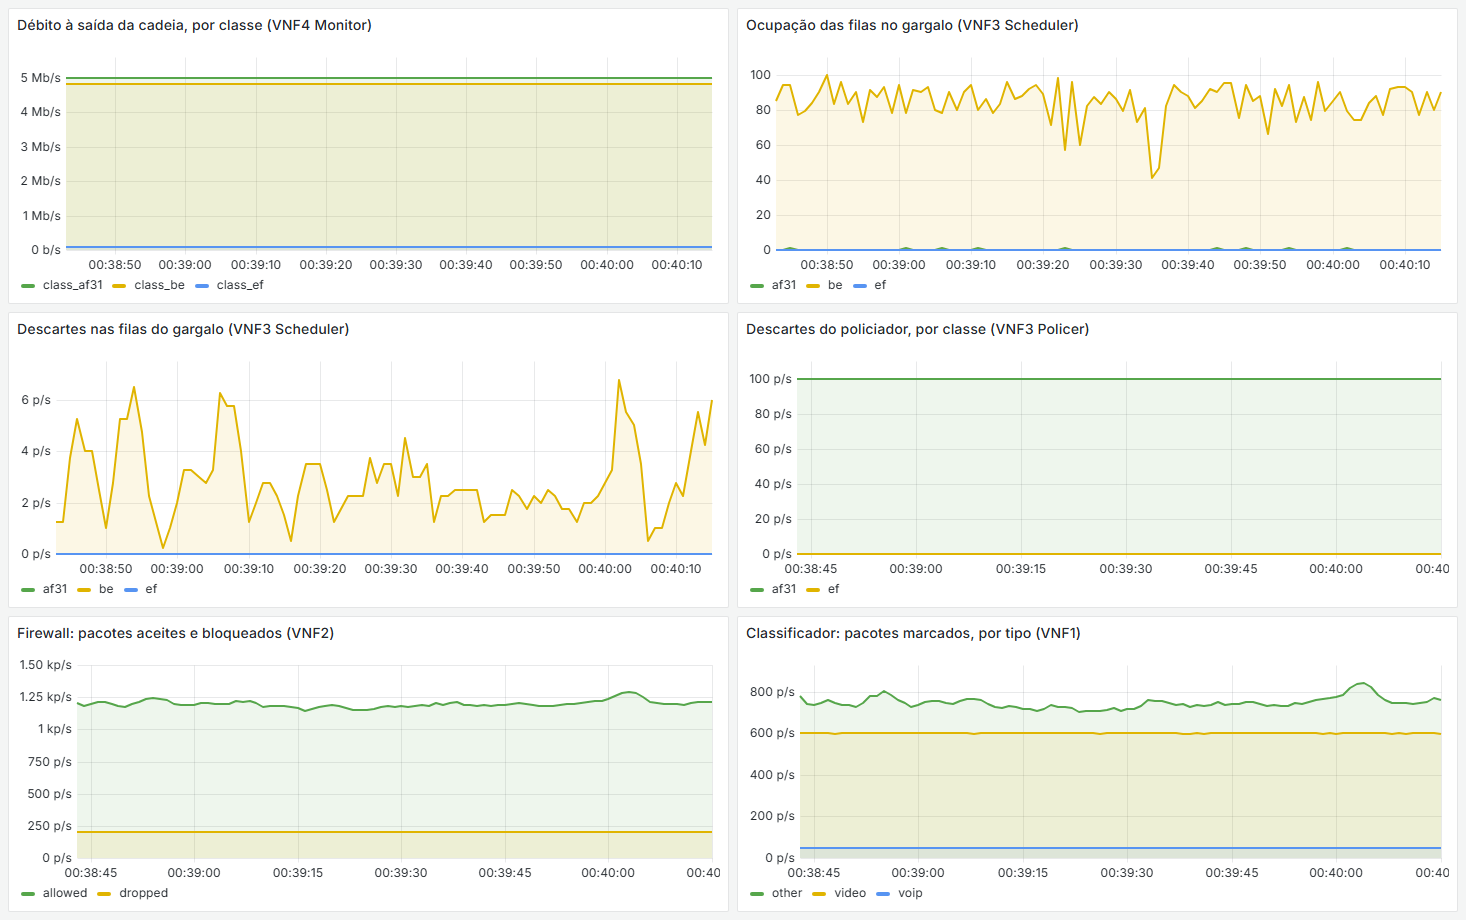
\includegraphics[width=0.7\textwidth]{grafana.png}
\caption{\emph{Dashboard} do Grafana com a cadeia completa, vídeo a 6~Mbit/s (acima do
perfil de 5~Mbit/s) e 2~Mbit/s de tráfego não autorizado. Vê-se o vídeo limitado a
5~Mbit/s, a fila de BE cheia e as de EF e AF31 vazias, 100~pacotes/s descartados pelo
policiador e 200~pacotes/s bloqueados pela firewall.}
\label{fig:grafana}
\end{figure}

\subsection{Geração de tráfego e medição ativa}

O tráfego TCP é gerado com o \texttt{iperf3}. Para o tráfego UDP foi escrito um
gerador próprio, o \texttt{udpgen}, que também mede: cada pacote leva um número de
sequência e o instante de envio, e o recetor calcula as métricas num sentido usadas na
UC. São elas o atraso (IPTD, ou OWD~\cite{rfc7679}), a variação do atraso entre
pacotes consecutivos (IPDV~\cite{rfc3393}), a razão de perdas (IPLR) e o débito. O
atraso num sentido exige normalmente relógios sincronizados; aqui, emissor e recetor
são contentores na mesma máquina e leem o mesmo relógio monotónico, pelo que não há
erro de sincronização. O gerador pode enviar a débito constante ou em rajadas de $N$
pacotes, para imitar os \emph{frames} de vídeo.

Para o VoIP estima-se ainda a qualidade percebida, com o MOS dado pelo modelo~E
simplificado de Cole e Rosenbluth~\cite{cole,g107} para o codec G.711: $R = 94{,}2 -
I_d - I_e$, em que $I_d$ cresce com o atraso boca-ouvido e $I_e$ com as perdas. Ao
atraso medido na rede somam-se 60~ms dos terminais (empacotamento e \emph{buffer} de
compensação de \emph{jitter}).

\section{Metodologia de avaliação}
\label{sec:met}

\subsection{Tráfego e configurações}

A Tabela~\ref{tab:trafego} resume o tráfego gerado. A mistura de referência é uma
chamada VoIP, um fluxo de vídeo e quatro fluxos TCP, que em conjunto excedem a
capacidade do gargalo; uma sonda UDP de 32~kbit/s mede o atraso da classe
\emph{best effort}. Os objetivos do VoIP são os da classe~0 da
Y.1541~\cite{y1541}.

\begin{table}[!tb]
\caption{Classes de tráfego, perfis gerados e objetivos de QoS.}
\label{tab:trafego}
\centering
\footnotesize
\begin{tabularx}{\textwidth}{@{}l Y l Y@{}}
\toprule
Aplicação & Perfil gerado & DSCP & Objetivo \\
\midrule
VoIP (G.711) & UDP, 50~pacotes/s de 200~B (80~kbit/s) & EF (46) &
  IPTD $\le$ 100~ms, IPDV $\le$ 50~ms, IPLR $\le 10^{-3}$ \\
Vídeo & UDP, 400~pacotes/s de 1250~B (4~Mbit/s) & AF31 (26) &
  Débito sustentado, IPLR $\le 10^{-3}$ \\
Dados em massa & TCP, 1 a 8 fluxos sem limite de débito & BE (0) &
  Sem garantias; usa a capacidade restante \\
Não autorizado & UDP a partir de h\_x, até 12~Mbit/s & --- & Bloqueado na VNF2 \\
\bottomrule
\end{tabularx}
\end{table}

Comparam-se cinco configurações, os perfis da Tabela~\ref{tab:perfis}. O perfil
\texttt{policeonly} não estava na proposta; foi acrescentado para separar o efeito do
policiamento do efeito do agendamento.

\begin{table}[!tb]
\caption{Perfis de teste: mecanismos ativos em cada configuração.}
\label{tab:perfis}
\centering
\footnotesize
\begin{tabularx}{\textwidth}{@{}l Y c c c c@{}}
\toprule
Perfil & Nome nos gráficos & Classif. & Firewall & Polic. & Agend. \\
\midrule
\texttt{baseline} & Sem QoS & & & & \\
\texttt{policeonly} & Só policiamento & $\bullet$ & & $\bullet$ & \\
\texttt{sched} & Agendamento & $\bullet$ & & & $\bullet$ \\
\texttt{police} & Agendamento + policiamento & $\bullet$ & & $\bullet$ & $\bullet$ \\
\texttt{full} & Cadeia completa & $\bullet$ & $\bullet$ & $\bullet$ & $\bullet$ \\
\bottomrule
\end{tabularx}
\end{table}

\subsection{Cenários e procedimento}

Cada VNF foi primeiro testada isoladamente, com as outras em modo de passagem
(Secção~\ref{sec:isoladas}). A avaliação da cadeia é feita por uma campanha de dez
cenários (Tabela~\ref{tab:cenarios}), que cobrem o que o enunciado pede: carga
variável, congestionamento, atraso, perdas e falhas, e a otimização de parâmetros.

\begin{table}[!tb]
\caption{Cenários da campanha. Salvo indicação, o tráfego é a mistura de referência.}
\label{tab:cenarios}
\centering
\footnotesize
\begin{tabularx}{\textwidth}{@{}l Y L{3.6cm}@{}}
\toprule
Cenário & Parâmetro que varia & Perfis comparados \\
\midrule
Carga & Fluxos TCP: 0, 1, 2, 4, 8 & Todos menos \texttt{policeonly} \\
Vídeo fora do perfil & Débito do vídeo: 4, 6, 8, 12~Mbit/s & Todos menos \texttt{full} \\
Tráfego não autorizado & Débito de h\_x: 0, 4, 8, 12~Mbit/s & \texttt{baseline}, \texttt{sched}, \texttt{full} \\
Atraso no núcleo & 5, 25, 50, 100~ms & \texttt{baseline}, \texttt{full} \\
Perdas no núcleo & 0, 0,5, 1, 2\% & \texttt{baseline}, \texttt{full} \\
Falha no núcleo & Falha de 3~s a meio da corrida & \texttt{baseline}, \texttt{full} \\
Tamanho das filas & 20, 50, 100, 300~pacotes & \texttt{sched} \\
Pesos das classes & AF31/BE: 3/6, 5/4, 7/2~Mbit/s; vídeo a 6~Mbit/s & \texttt{sched} \\
Balde do policiador & 5, 10, 20, 40, 100~kB; vídeo em rajadas & \texttt{police} \\
Sobrecarga & Sem gargalo: encaminhamento direto ou pela cadeia & direto, \texttt{baseline}, \texttt{full} \\
\bottomrule
\end{tabularx}
\end{table}

Cada ponto é medido em cinco corridas independentes de 60~s, num total de
420~corridas e cerca de oito horas. Os fluxos TCP arrancam 1,5~s antes dos restantes,
para a fila já estar cheia quando a medição começa. O débito TCP é a média sobre toda
a duração do fluxo, que inclui esses instantes sem tráfego UDP: fica sobrestimado em
0,1 a 0,3~Mbit/s e, onde se lê cerca de 0,3~Mbit/s, o débito durante a contenção é
praticamente nulo. Os gráficos mostram a média das
cinco corridas e o intervalo de confiança de 95\%, calculado com a distribuição $t$ de
Student. Um único comando (\texttt{make experiments SET=full}) corre a campanha, que
pode ser interrompida e retomada, e gera os gráficos e a tabela-resumo a partir do
ficheiro com uma linha por fluxo e por corrida.

\section{Resultados}
\label{sec:res}

\subsection{VNFs isoladas}
\label{sec:isoladas}

O comando \texttt{make test} ativa uma VNF de cada vez e faz 26~verificações
automáticas, todas satisfeitas. O \texttt{traceroute} de um cliente para um servidor
passa pelas quatro VNFs, pela ordem configurada. À saída da VNF1, o VoIP tem o campo
ToS a \texttt{0xb8}~(EF), o vídeo a \texttt{0x68}~(AF31), e um pacote que o cliente
marcou como EF sem ser VoIP é remarcado para~0. A firewall deixa passar os clientes
autorizados e bloqueia o \texttt{h\_x} e as portas fora da lista. O policiador não
causa perdas ao VoIP dentro do perfil e limita uma fonte de 400~kbit/s a 216~kbit/s;
o valor fica acima dos 200~kbit/s contratados porque o balde começa cheio e, num
teste de 5~s, os seus 10~kB valem mais 16~kbit/s.

\subsection{Carga crescente}

A Fig.~\ref{fig:load} mostra o efeito do número de fluxos TCP, e a
Tabela~\ref{tab:carga} detalha o ponto com quatro fluxos. Sem QoS, basta um fluxo TCP
para encher a fila única do gargalo. O atraso do VoIP sobe de 5~ms para 109~ms, o
valor previsto pela configuração: uma fila de 100~pacotes de 1500~B demora $100
\times 1500 \times 8 / 10^7 = 120$~ms a esvaziar a 10~Mbit/s. Os objetivos da classe~0
da Y.1541 deixam de ser cumpridos: o atraso médio fica entre 94 e 102~ms, no limite
dos 100~ms, e as perdas do VoIP (entre 0,3\% e 1,1\%) excedem $10^{-3}$. A amplitude
do atraso, medida entre o mínimo e o percentil~99, anda entre 33 e 55~ms.

\begin{figure}[!tb]
\centering
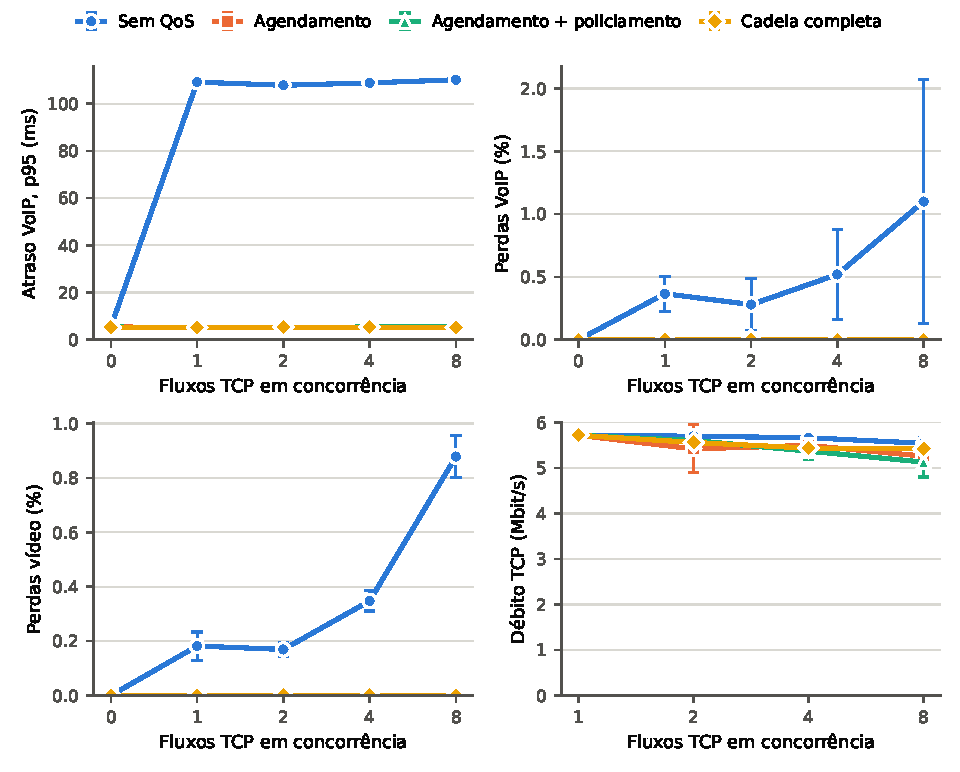
\includegraphics[width=\textwidth]{load.pdf}
\caption{Carga crescente: VoIP, vídeo e TCP em função do número de fluxos TCP.}
\label{fig:load}
\end{figure}

\begin{table}[!tb]
\caption{VoIP e vídeo em concorrência com quatro fluxos TCP: média de cinco corridas
de 60~s e intervalo de confiança de 95\%. Atrasos em ms e débito em Mbit/s.}
\label{tab:carga}
\centering
\footnotesize
\begin{tabular*}{\textwidth}{@{\extracolsep{\fill}}l r r r r r@{}}
\toprule
 & \multicolumn{3}{c}{VoIP} & Vídeo & TCP \\
\cmidrule{2-4}
Configuração & IPTD p95 & IPDV & IPLR & IPLR & Débito \\
\midrule
Sem QoS & 108,8 $\pm$ 0,5 & 5,61 & 0,52\% & 0,35\% & 5,66 $\pm$ 0,04 \\
Agendamento & 5,3 $\pm$ 0,1 & 0,08 & 0\% & 0\% & 5,49 $\pm$ 0,17 \\
Agendamento + policiamento & 5,4 $\pm$ 0,1 & 0,10 & 0\% & 0\% & 5,37 $\pm$ 0,18 \\
Cadeia completa & 5,4 $\pm$ 0,1 & 0,09 & 0\% & 0\% & 5,43 $\pm$ 0,08 \\
\bottomrule
\end{tabular*}
\end{table}

Com classificação e agendamento, o VoIP e o vídeo ficam isolados da carga. O atraso do
VoIP mantém-se em 5,3~ms, que é o atraso do núcleo, tanto com um fluxo TCP como com
oito; a amplitude do atraso fica abaixo de 0,5~ms e não há perdas em VoIP nem em
vídeo em nenhuma das corridas. O TCP continua a usar a capacidade que sobra: com a
cadeia completa obtém 5,43~Mbit/s, menos 4\% do que sem QoS. A diferença não vem do
tráfego prioritário, que ocupa o mesmo nos dois casos, mas da fila própria da classe
BE, onde o atraso sentido pelo TCP duplica: com filas de 50~pacotes, o TCP obtém o
mesmo débito que sem QoS (Secção~\ref{sec:otim}).

\subsection{Fonte de vídeo fora do perfil}

Neste cenário, a fonte de vídeo envia mais do que os 5~Mbit/s contratados
(Fig.~\ref{fig:policing}). Sem QoS, quem envia mais fica com mais: a 12~Mbit/s, o
vídeo ocupa 9,8~Mbit/s, o TCP fica reduzido a 0,34~Mbit/s e o VoIP perde 52\% dos
pacotes. É a falta de equidade de uma fila única perante uma fonte que não reage ao
congestionamento.

\begin{figure}[!tb]
\centering
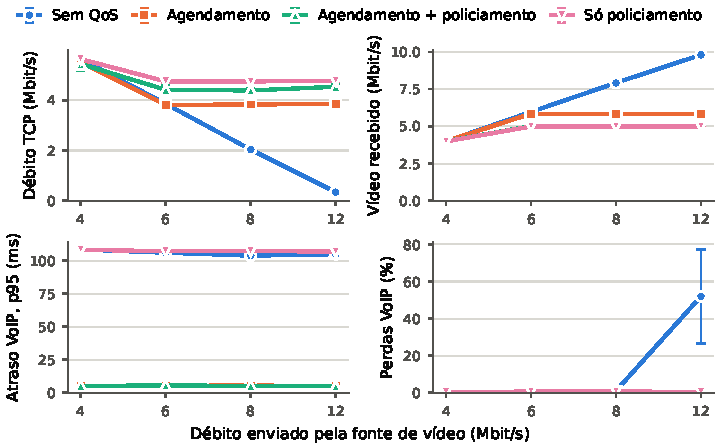
\includegraphics[width=\textwidth]{policing.pdf}
\caption{Fonte de vídeo que excede o perfil contratado de 5~Mbit/s.}
\label{fig:policing}
\end{figure}

Os três perfis com QoS mostram que o policiamento e o agendamento se completam:

\begin{itemize}
\item \textbf{Só policiamento.} O vídeo é limitado a 5,0~Mbit/s e o TCP mantém
4,8~Mbit/s, mas a fila continua a ser única: o atraso do VoIP continua em 107~ms e a
sua variação (IPDV) entre 4,7 e 5,4~ms, da mesma ordem que sem QoS, contra menos de
0,1~ms com agendamento. O policiamento garante equidade, não garante atraso nem \emph{jitter}.
\item \textbf{Só agendamento.} O VoIP fica protegido (5,3~ms, sem perdas). O vídeo
obtém 5,85~Mbit/s, porque a classe AF31 tem prioridade sobre BE na capacidade que
sobra, e o TCP fica nos 3,8~Mbit/s garantidos. Mas a fila de AF31 está sempre cheia,
e o próprio vídeo passa a ter 176~ms de atraso.
\item \textbf{Os dois.} O excesso é descartado à entrada, antes de chegar à fila. O
vídeo que passa (5,0~Mbit/s) tem 6~ms de atraso, e o TCP sobe para 4,4 a 4,5~Mbit/s.
\end{itemize}

O compromisso é o que o enunciado sugere: o policiamento reduz o débito de quem
excede o contrato (a 12~Mbit/s, 58\% dos pacotes de vídeo são descartados) e, em
troca, protege os outros fluxos e mantém baixo o atraso do tráfego conforme.

\subsection{Tráfego não autorizado}

A Fig.~\ref{fig:flood} mostra o efeito de tráfego UDP enviado por \texttt{h\_x}, que
não é um cliente autorizado. Sem QoS, 12~Mbit/s desse tráfego bastam para o VoIP
perder 61\% dos pacotes, o vídeo 58\% e o TCP ficar com 0,29~Mbit/s. O agendamento,
sozinho, protege o VoIP e o vídeo, mas não o TCP: o tráfego de \texttt{h\_x} é
classificado como \emph{best effort} e compete com o TCP na mesma classe, onde ganha
por não reagir às perdas. Só com a firewall, que o descarta na VNF2, o débito TCP se
mantém em 5,5~Mbit/s, qualquer que seja o débito do ataque.

\begin{figure}[!tb]
\centering
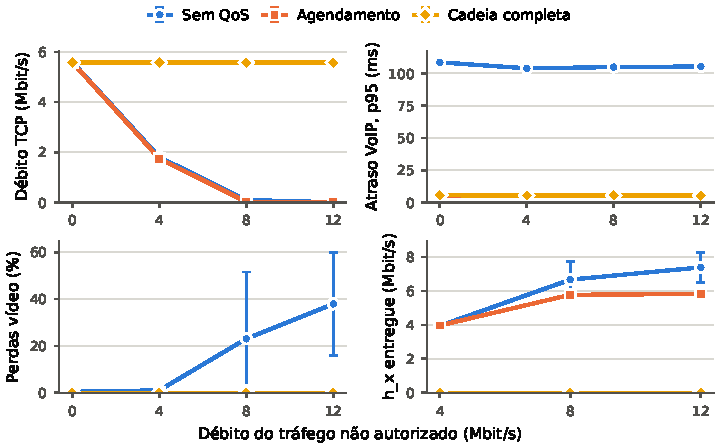
\includegraphics[width=\textwidth]{flood.pdf}
\caption{Tráfego UDP não autorizado, enviado por h\_x.}
\label{fig:flood}
\end{figure}

\subsection{Qualidade percebida do VoIP}

A Fig.~\ref{fig:mos} traduz os resultados dos dois cenários anteriores em MOS
estimado. Com a cadeia, o MOS é 4,40 em todos os cenários de carga, que é o máximo do
modelo para os 65~ms de atraso boca-ouvido. Sem QoS há dois regimes. Só com carga
TCP, o MOS desce pouco (4,2 a 4,3 no cenário de carga crescente), porque o modelo~E
só penaliza fortemente o atraso acima de 177~ms e as perdas são da ordem de 1\%.
Quando o tráfego UDP excede a capacidade, as perdas dominam e a chamada deixa de ser
utilizável: o MOS é 1,5 com o vídeo a 12~Mbit/s e 1,3 com 12~Mbit/s de tráfego não
autorizado.

\begin{figure}[!tb]
\centering
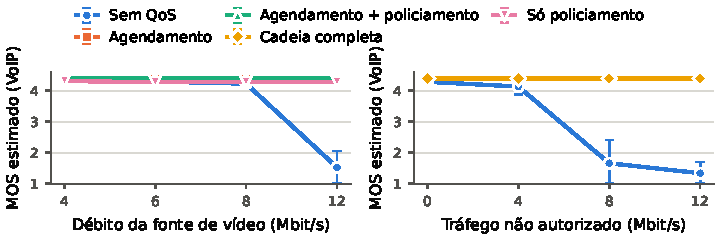
\includegraphics[width=\textwidth]{mos.pdf}
\caption{MOS estimado do VoIP (modelo~E simplificado, codec G.711) com vídeo fora do
perfil e com tráfego não autorizado.}
\label{fig:mos}
\end{figure}

\subsection{Condições do núcleo: atraso, perdas e falha}

Os mecanismos de QoS estão no acesso; estes cenários mostram o que eles conseguem, e
não conseguem, quando o problema está no núcleo (Tabela~\ref{tab:nucleo}). O atraso
do núcleo soma-se sempre, mas sem QoS soma-se ao atraso da fila: com 100~ms no
núcleo, o VoIP tem 100~ms com a cadeia e 202~ms sem ela, já acima do limiar a partir
do qual o modelo~E penaliza a conversação. As perdas do núcleo acontecem depois da
cadeia e afetam as duas configurações por igual; nenhum mecanismo no acesso as pode
corrigir.

\begin{table}[!tb]
\caption{VoIP com quatro fluxos TCP, em função das condições da ligação ao núcleo.}
\label{tab:nucleo}
\centering
\footnotesize
\begin{tabular*}{\textwidth}{@{\extracolsep{\fill}}l r r r r r r r r@{}}
\toprule
 & \multicolumn{4}{c}{IPTD p95 (ms), por atraso} &
   \multicolumn{4}{c}{IPLR (\%), por perdas} \\
\cmidrule{2-5}\cmidrule{6-9}
Configuração & 5~ms & 25~ms & 50~ms & 100~ms & 0\% & 0,5\% & 1\% & 2\% \\
\midrule
Sem QoS & 108,3 & 127,9 & 152,8 & 201,6 & 0,35 & 0,79 & 1,06 & 1,90 \\
Cadeia completa & 5,5 & 25,5 & 50,4 & 100,3 & 0,00 & 0,51 & 1,05 & 1,98 \\
\bottomrule
\end{tabular*}
\end{table}

Na falha temporária (Fig.~\ref{fig:outage}), a ligação ao núcleo é cortada durante
3~s a meio da corrida. Os pacotes enviados durante a falha perdem-se nos dois casos
(5\% dos pacotes da corrida). A diferença está na recuperação: com a cadeia, o VoIP
retoma de imediato os 5~ms; sem QoS, tem dois a três segundos de atraso baixo,
enquanto o TCP ainda está em recuo exponencial, e volta aos 100~ms assim que o TCP
recupera.

\begin{figure}[!tb]
\centering
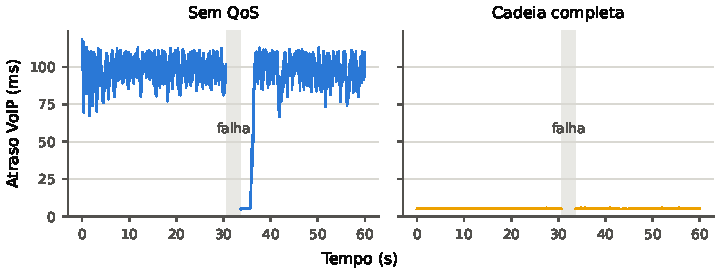
\includegraphics[width=\textwidth]{outage.pdf}
\caption{Atraso do VoIP ao longo de uma corrida com uma falha de 3~s na ligação ao núcleo.}
\label{fig:outage}
\end{figure}

\subsection{Otimização dos parâmetros}
\label{sec:otim}

\subsubsection{Tamanho das filas.}
A Fig.~\ref{fig:queue} mostra o efeito do tamanho das filas das classes HTB. O atraso
da classe \emph{best effort} cresce em proporção com a fila, de 44~ms (p95) com
20~pacotes para 592~ms com 300, e o débito TCP não melhora: é 5,7~Mbit/s com 20 ou
50~pacotes e 5,3 a 5,4~Mbit/s com 100 ou 300. Filas grandes só acrescentam atraso. No
outro extremo, com 20~pacotes a sonda \emph{best effort} perde 2,7\% dos pacotes,
contra menos de 1\% nos outros casos. O melhor compromisso está nos 50~pacotes. O
VoIP não depende deste parâmetro: tem a sua própria fila, que nunca enche.

\begin{figure}[!tb]
\centering
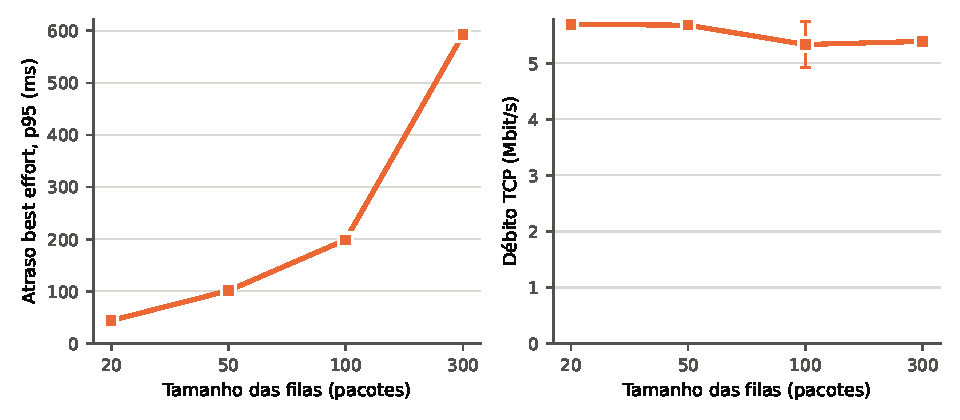
\includegraphics[width=\textwidth]{queue.pdf}
\caption{Otimização: tamanho das filas das classes (perfil \texttt{sched}).}
\label{fig:queue}
\end{figure}

\subsubsection{Pesos das classes.}
No HTB, os débitos garantidos de AF31 e BE funcionam como pesos na partilha do
gargalo. A Fig.~\ref{fig:weights} mostra três repartições, com o vídeo a 6~Mbit/s.
Com 3~Mbit/s garantidos a AF31, o vídeo perde 35\% dos pacotes e o TCP fica com
5,6~Mbit/s. Com 5~Mbit/s, as perdas descem para 2,2\%: a classe ainda recebe o que
sobra de EF, mas não chega para os 6~Mbit/s. Com 7~Mbit/s não há perdas e o atraso do
vídeo desce de 176~ms para 5~ms, à custa do TCP, que fica com 3,6~Mbit/s. A regra que
daqui resulta é simples: o débito garantido de uma classe deve cobrir o perfil
contratado para ela, e o policiador deve impedir que esse perfil seja excedido. É o
que faz a configuração de referência (5~Mbit/s nos dois).

\begin{figure}[!tb]
\centering
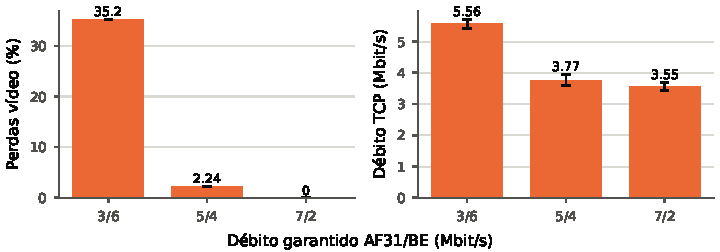
\includegraphics[width=\textwidth]{weights.pdf}
\caption{Otimização: débitos garantidos de AF31 e BE, com vídeo a 6~Mbit/s (perfil
\texttt{sched}).}
\label{fig:weights}
\end{figure}

\subsubsection{Tamanho do balde do policiador.}
Um fluxo de vídeo real não tem débito constante: envia os pacotes de cada
\emph{frame} de seguida. Neste cenário, o vídeo mantém os 4~Mbit/s, dentro do perfil,
mas em rajadas de 16~pacotes (um \emph{frame} de 20~kB a cada 40~ms). A
Fig.~\ref{fig:bucket} mostra que o balde do policiador tem de comportar a rajada: com
5~kB só passam 4 dos 16~pacotes de cada \emph{frame} (75\% de perdas), com 10~kB
passam 8 (50\%), e a partir de 20~kB não há perdas. Um balde demasiado pequeno
castiga tráfego que cumpre o débito contratado. Um balde demasiado grande tem o
defeito oposto: deixa passar de uma vez rajadas maiores, como no teste isolado. A escolha
deve ser a maior rajada legítima do tráfego, com alguma margem. As rajadas têm também
um custo a jusante: os pacotes de um \emph{frame} esperam uns pelos outros na fila de
AF31, e o atraso do vídeo sobe de 5~ms para 31~ms (p95).

\begin{figure}[!tb]
\centering
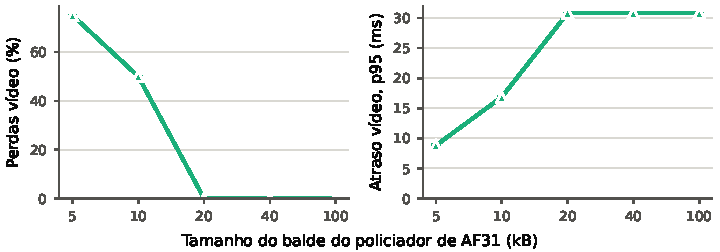
\includegraphics[width=\textwidth]{bucket.pdf}
\caption{Otimização: tamanho do balde do policiador de AF31, com vídeo de 4~Mbit/s em
rajadas de 20~kB (perfil \texttt{police}).}
\label{fig:bucket}
\end{figure}

\subsection{Sobrecarga da cadeia}

Para medir o custo da virtualização, retirou-se o limite de 10~Mbit/s e o atraso do
núcleo e comparou-se a cadeia com o encaminhamento direto, sem VNFs
(Fig.~\ref{fig:overhead}). Um fluxo TCP atinge 8,7~Gbit/s em encaminhamento direto,
3,1~Gbit/s através da cadeia em modo de passagem e 2,8~Gbit/s com a cadeia completa.
A maior parte do custo vem, portanto, de atravessar mais quatro nós; as regras de QoS
propriamente ditas custam cerca de 9\%. No atraso, com carga, a cadeia acrescenta
0,03 a 0,04~ms. Sem carga, os atrasos medidos são maiores (cerca de 0,5~ms) e a
ordem entre configurações não é significativa: domina o tempo que o processador,
em repouso, demora a acordar para tratar cada pacote.

\begin{figure}[!tb]
\centering
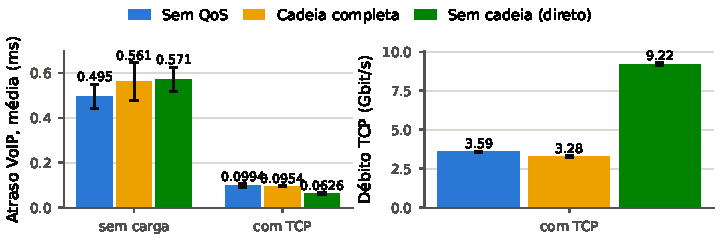
\includegraphics[width=\textwidth]{overhead.pdf}
\caption{Sobrecarga da cadeia, sem gargalo: atraso do VoIP e débito de um fluxo TCP.}
\label{fig:overhead}
\end{figure}

Os valores absolutos dependem da máquina; para um acesso de 10~Mbit/s, a cadeia tem
capacidade 280~vezes superior à necessária.

\section{Discussão}
\label{sec:disc}

\subsection{O contributo de cada mecanismo}

Os resultados permitem atribuir a cada VNF um papel distinto, que nenhuma das outras
substitui. A \emph{classificação} não melhora nada por si só, mas é a condição dos
restantes mecanismos: sem a marca DSCP, o policiador e o scheduler não distinguem os
fluxos. O \emph{agendamento} é o que garante o atraso: é o único mecanismo que retira
o VoIP da fila partilhada. O \emph{policiamento} garante a equidade e mantém baixo o
atraso do tráfego conforme, quando uma fonte excede o seu perfil. O \emph{controlo de
acesso} protege a classe \emph{best effort}, que os outros mecanismos deixam exposta.
A \emph{monitorização} não altera o tráfego, mas foi o que permitiu verificar cada
um destes efeitos e detetar erros de configuração durante o desenvolvimento.

Os compromissos medidos são os clássicos do DiffServ. Separar as classes custa
ao TCP 4\% do débito, com as filas de referência. Policiar custa perdas a quem excede o contrato. Aumentar o
débito garantido de uma classe retira-o às outras. Aumentar as filas troca perdas por
atraso. Em nenhum caso há ganho sem custo; o que os mecanismos fazem é escolher quem
paga, e essa escolha passa a estar num ficheiro de configuração.

\subsection{VNFs face a abordagens não virtualizadas}

Os mecanismos usados são os de um encaminhador tradicional: listas de acesso,
\emph{token buckets} e filas por classe. O que muda com a virtualização é a forma
como são disponibilizados.

\begin{itemize}
\item \textbf{Flexibilidade.} Mudar de perfil é voltar a correr quatro \emph{scripts},
sem interromper a topologia; trocar a ordem das VNFs ou acrescentar uma é editar uma
lista.
Num equipamento dedicado, as funções disponíveis e a sua ordem são as que o
fabricante definiu.
\item \textbf{Independência.} Cada função é uma imagem que pode ser atualizada,
substituída ou escalada sem tocar nas outras. Juntar o policiamento e o agendamento
na VNF3 poupou um salto, à custa de parte dessa independência.
\item \textbf{Reprodutibilidade.} Todo o sistema, incluindo a rede, é descrito por
ficheiros e criado por comandos. As experiências deste relatório repetem-se num
computador portátil, o que não seria possível com equipamento físico.
\item \textbf{Custo.} A virtualização paga-se em desempenho: a cadeia reduz o débito
máximo a cerca de um terço. É irrelevante no acesso e relevante no núcleo, onde os
equipamentos dedicados encaminham em \emph{hardware}. As respostas habituais são
acelerar o plano de dados (DPDK, XDP, SR-IOV) ou distribuir a carga por várias
instâncias.
\end{itemize}

\subsection{Escalabilidade e limitações}

A cadeia é em série: cada VNF é um ponto único de falha e o débito máximo é o da VNF
mais lenta. Escalar horizontalmente é possível para a classificação e para o
policiamento, repartindo os fluxos por instâncias. É mais difícil para a firewall,
que guarda o estado das ligações, e para o scheduler, que tem de ver todo o tráfego
da ligação que gere. O orquestrador deste trabalho é deliberadamente mínimo: cria e
configura a cadeia, mas não vigia as VNFs, não as relança nem as escala. Essas
funções existem em plataformas como o OSM ou o Kubernetes.

A avaliação tem limitações que convém ter presentes. É uma emulação numa só máquina,
pelo que os valores absolutos de sobrecarga não se transpõem para outro
\emph{hardware}. O tráfego é sintético, com um só gargalo e fontes UDP que não reagem
ao congestionamento. A classificação é feita por portas e não distingue aplicações
que as partilhem, e a cadeia só trata o sentido dos clientes para os servidores. O MOS
é uma estimativa, e não uma medida subjetiva.

\section{Conclusão}
\label{sec:conc}

Implementou-se uma cadeia de quatro VNFs que cobre os cinco aspetos de QoS do
enunciado e avaliou-se com uma campanha automática e reprodutível de 420~corridas. Num gargalo de 10~Mbit/s com
tráfego TCP concorrente, a cadeia reduz o atraso do VoIP de 109~ms para 5~ms e
elimina as perdas em VoIP e vídeo, com um custo de 4\% no débito TCP. Perante uma
fonte de vídeo ou tráfego não autorizado a 12~Mbit/s, o MOS do VoIP mantém-se em
4,4, quando sem QoS desce para 1,5 e 1,3.

A principal lição é que os mecanismos se completam: o agendamento garante o atraso,
o policiamento a equidade e o controlo de acesso protege a classe sem garantias. A
otimização deu regras simples para os parâmetros: filas curtas, débitos garantidos
iguais ao perfil contratado e baldes à medida da maior rajada legítima. A
virtualização custa dois terços do débito máximo, um preço irrelevante no acesso.

Como trabalho futuro, propõe-se uma plataforma de orquestração que vigie e escale
as VNFs, gestão ativa de filas na classe \emph{best effort} e tráfego real.

\begin{thebibliography}{[14}
\makeatletter\renewcommand\@biblabel[1]{[#1]}\makeatother  % etiquetas [n], como no estilo IEEE
\bibitem{etsi-nfv} ETSI, ``Network Functions Virtualisation (NFV); Architectural Framework,'' ETSI GS NFV 002 V1.2.1, 2014.
\bibitem{rfc2475} S. Blake \emph{et al.}, ``An architecture for differentiated services,'' RFC 2475, IETF, 1998.
\bibitem{containernet} M. Peuster, H. Karl, and S. van Rossem, ``MeDICINE: Rapid prototyping of production-ready network services in multi-PoP environments,'' in \emph{Proc. IEEE NFV-SDN}, 2016, pp. 148--153.
\bibitem{mininet} B. Lantz, B. Heller, and N. McKeown, ``A network in a laptop: Rapid prototyping for software-defined networks,'' in \emph{Proc. ACM HotNets-IX}, 2010.
\bibitem{rfc7665} J. Halpern and C. Pignataro, Eds., ``Service function chaining (SFC) architecture,'' RFC 7665, IETF, 2015.
\bibitem{rfc4594} J. Babiarz, K. Chan, and F. Baker, ``Configuration guidelines for DiffServ service classes,'' RFC 4594, IETF, 2006.
\bibitem{htb} M. Devera, ``HTB Linux queuing discipline manual -- user guide,'' 2002. [Online]. Available: \texttt{http://luxik.cdi.cz/\textasciitilde devik/qos/htb/manual/userg.htm}
\bibitem{rfc3246} B. Davie \emph{et al.}, ``An expedited forwarding PHB (per-hop behavior),'' RFC 3246, IETF, 2002.
\bibitem{rfc2597} J. Heinanen, F. Baker, W. Weiss, and J. Wroclawski, ``Assured forwarding PHB group,'' RFC 2597, IETF, 1999.
\bibitem{rfc7679} G. Almes, S. Kalidindi, M. Zekauskas, and A. Morton, Ed., ``A one-way delay metric for IP performance metrics (IPPM),'' RFC 7679, IETF, 2016.
\bibitem{rfc3393} C. Demichelis and P. Chimento, ``IP packet delay variation metric for IP performance metrics (IPPM),'' RFC 3393, IETF, 2002.
\bibitem{cole} R. G. Cole and J. H. Rosenbluth, ``Voice over IP performance monitoring,'' \emph{ACM SIGCOMM Comput. Commun. Rev.}, vol. 31, no. 2, pp. 9--24, 2001.
\bibitem{g107} ITU-T, ``The E-model: a computational model for use in transmission planning,'' Rec. G.107, 2015.
\bibitem{y1541} ITU-T, ``Network performance objectives for IP-based services,'' Rec. Y.1541, 2011.
\end{thebibliography}

\end{document}
